\documentclass{article}

\usepackage{graphicx}
\usepackage{tikz}
\usepackage{tikzsymbols}
\usetikzlibrary{calc,patterns,shapes.geometric}
\pagestyle{empty}
\usepackage[margin=0pt]{geometry}
\geometry{papersize={14in,12in}}

\def\centerarc[#1](#2)(#3:#4:#5){\draw[#1] ($(#2)+({#5*cos(#3)},{#5*sin(#3)})$) arc (#3:#4:#5);}

\begin{document}
	\begin{figure}
		\centering
		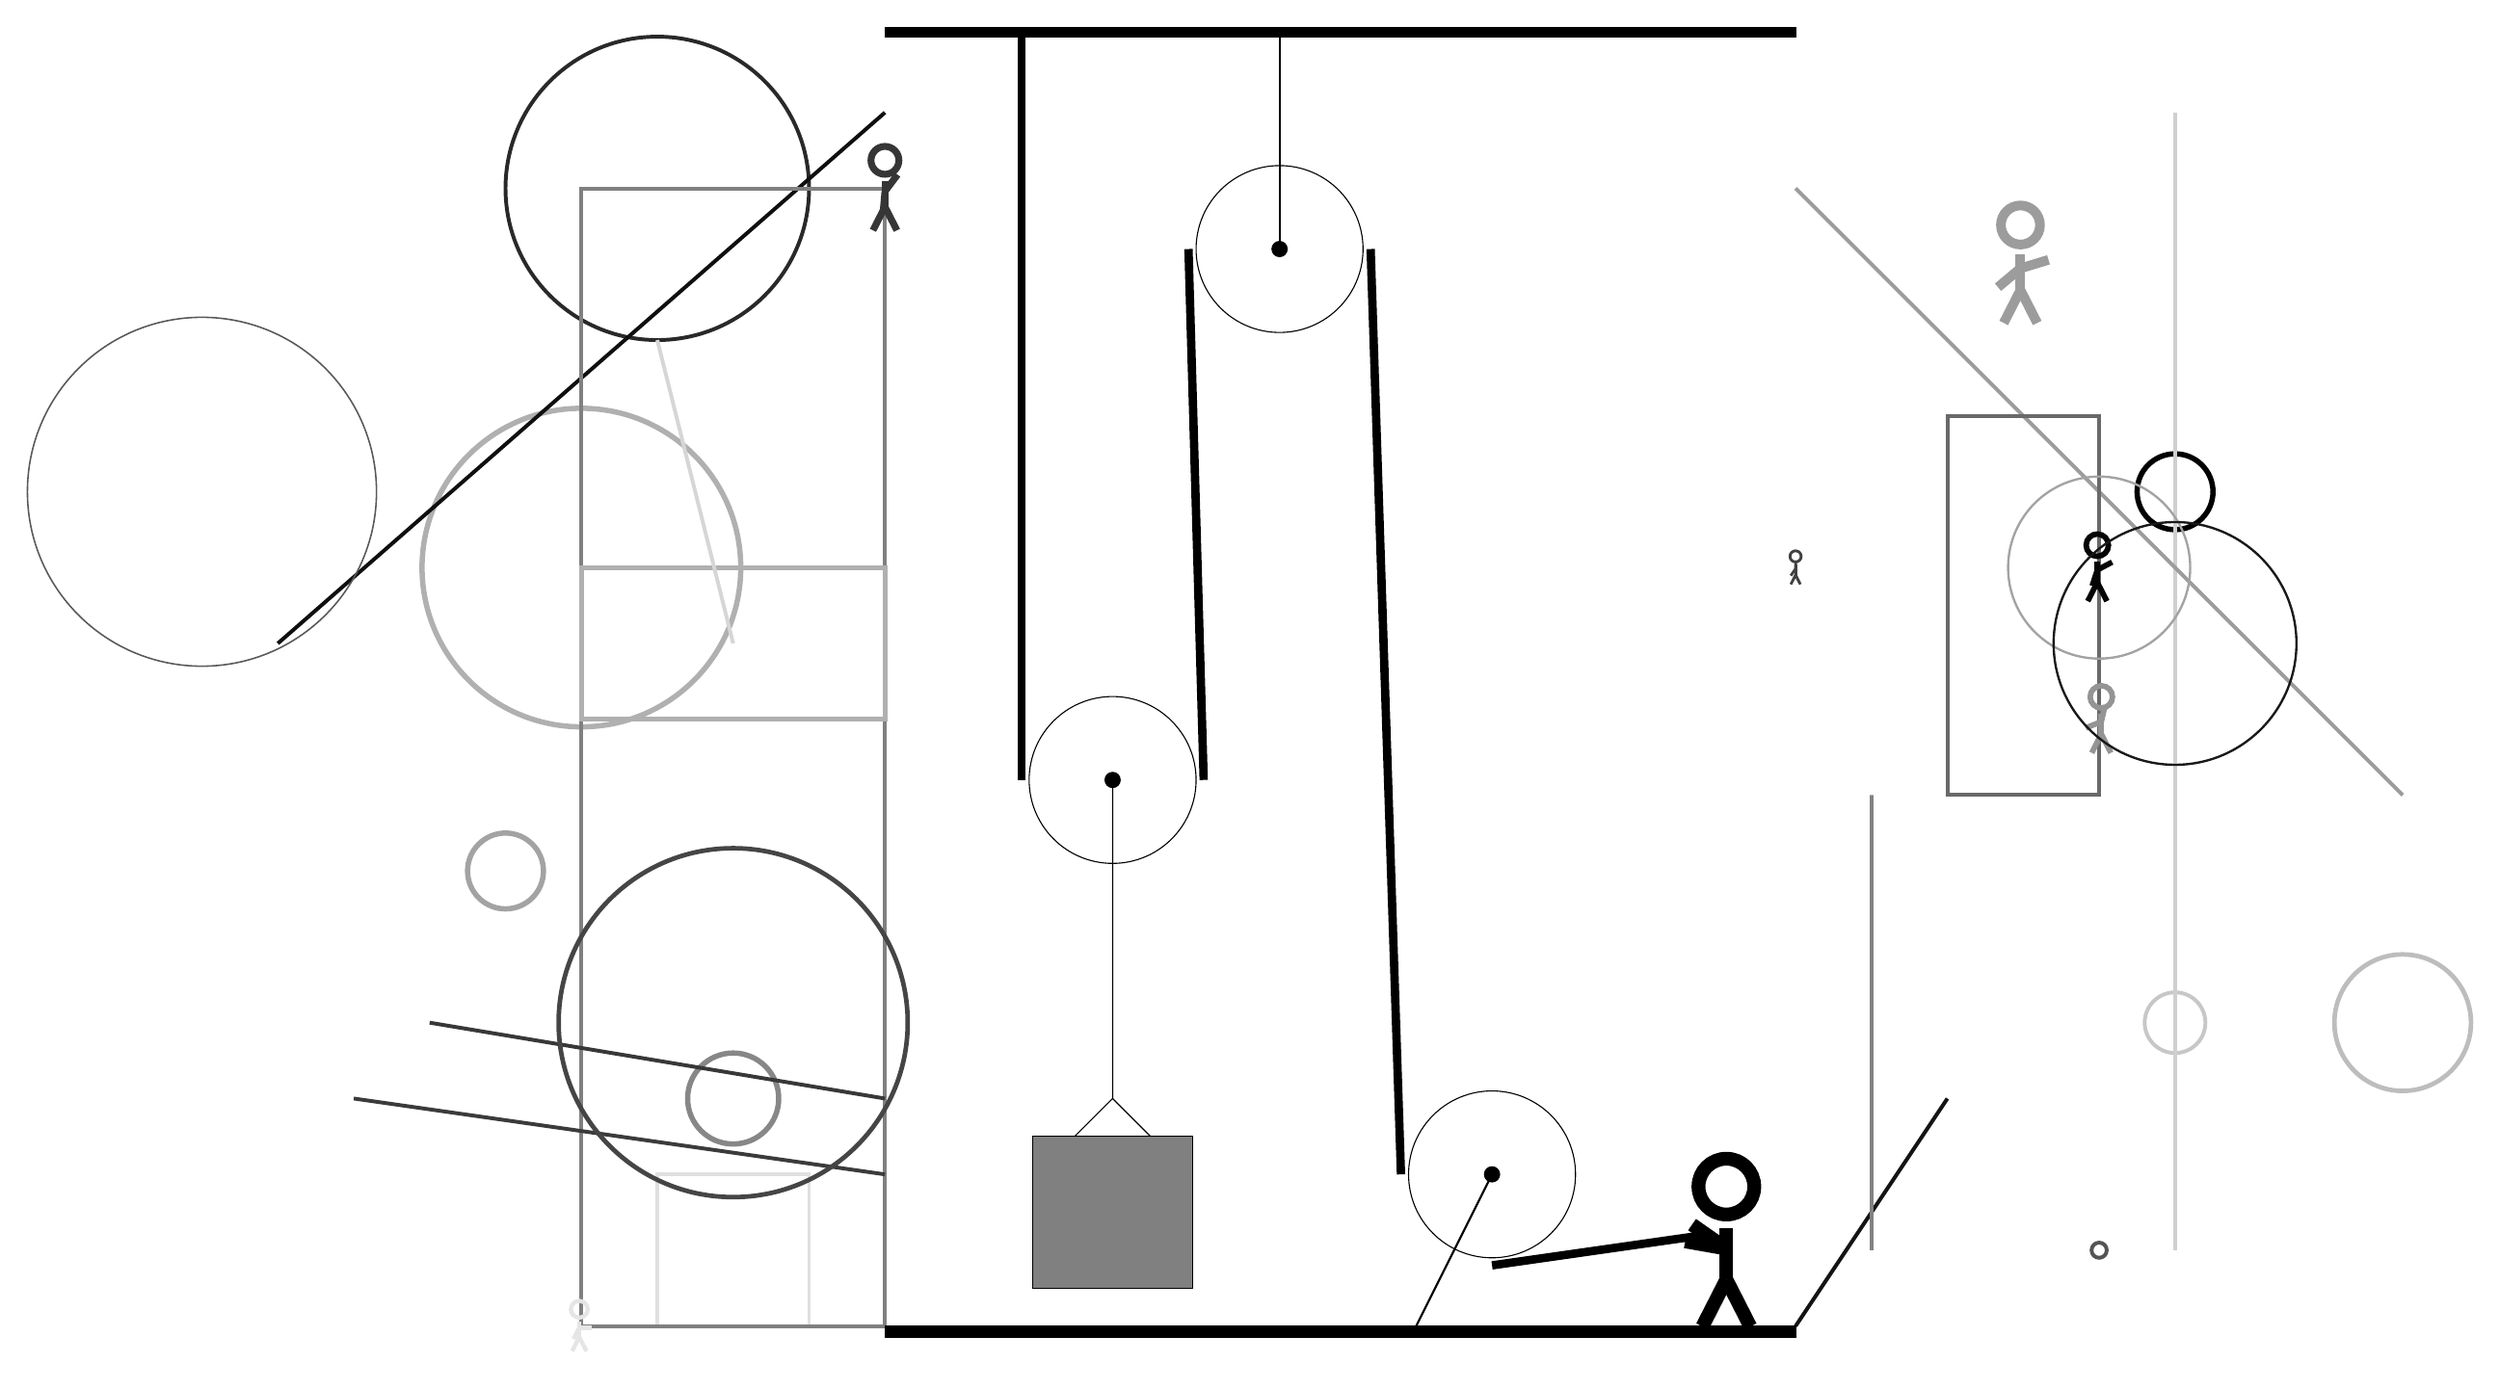
\begin{tikzpicture}
			%%%%% START %%%%%
			
			\draw[fill=black] (-2, 14) rectangle (10, 14.125);
			
			\draw (3.2, 11.2) circle (1.1);
			\draw[fill=black] (3.2, 11.2) circle (0.1);
			\draw[thick] (3.2, 11.2) -- (3.2, 14);
			
			\draw [line width=0.7mm, color=black!47](-4, 0) circle (0.6);
			
			\draw [line width=0.7mm, color=black!100](15, 8) circle (0.5);
			\node[line width=0.6mm, color=black!75] at (10, 7) {\Strichmaxerl[2][55][89]};
			\draw [line width=0.5mm, color=black!22](15, 1) circle (0.4);
			
			\draw [line width=0.6mm, color=black!26](18, 1) circle (0.9);
			\draw [line width=0.5mm, color=black!84](-5, 12) circle (2.0);
			
			\draw[line width=0.5mm, color=black!19](15, 13) -- (15, -2);
			\draw [line width=0.7mm, color=black!31](-6, 7) circle (2.1);
			\draw[line width=0.5mm, color=black!12] (-3, -3) rectangle (-5, -1);
			\draw[line width=0.5mm, color=black!39](10, 12) -- (18, 4);
			
			\draw[line width=0.5mm, color=black!94](-2, 13) -- (-10, 6);
			\draw[line width=0.5mm, color=black!59] (12, 9) rectangle (14, 4);
			\node[line width=0.3mm, color=black!39] at (13, 11) {\Strichmaxerl[7][40][17]};
			
			\draw[line width=0.5mm, color=black!50] (-2, -3) rectangle (-6, 12);
			\draw[line width=0.6mm, color=black!31] (-2, 7) rectangle (-6, 5);
			\draw[line width=0.5mm, color=black!92](10, -3) -- (12, 0);
			\node[line width=0.5mm, color=black!98] at (14, 7) {\Strichmaxerl[4][72][28]};
			\node[line width=0.6mm, color=black!42] at (14, 5) {\Strichmaxerl[4][22][77]};
			\draw [line width=0.2mm, color=black!65](-11, 8) circle (2.3);
			\draw[line width=0.5mm, color=black!77](-2, -1) -- (-9, 0);
			\draw[line width=0.5mm, color=black!78](-2, 0) -- (-8, 1);
			
			\draw [line width=0.5mm, color=black!67](14, -2) circle (0.1);
			\draw [line width=0.3mm, color=black!36](14, 7) circle (1.2);
			\draw [line width=0.6mm, color=black!73](-4, 1) circle (2.3);
			\node[line width=0.6mm, color=black!10] at (-6, -3) {\Strichmaxerl[3][62][0]};
			
			\draw [line width=0.3mm, color=black!90](15, 6) circle (1.6);
			
			\draw[line width=0.5mm, color=black!16](-5, 10) -- (-4, 6);
			\node[line width=0.6mm, color=black!79] at (-2, 12) {\Strichmaxerl[5][85][53]};
			\draw [line width=0.7mm, color=black!36](-7, 3) circle (0.5);
			\draw[line width=0.5mm, color=black!49] (11, -2) rectangle (11, 4);
			
			\draw (6, -1) circle (1.1);
			\draw[fill=black] (6, -1) circle (0.1);
			\draw[thick] (6, -1) -- (5, -3);
			
			\draw (1, 4.2) circle (1.1);
			\draw[fill=black] (1, 4.2) circle (0.1);
			
			\draw (1, 4.2) -- (1, 0) -- (0.5, -0.5);
			\draw (1, 0) -- (1.5, -0.5);
			\draw[fill=black!50] (-0.05, -0.5) rectangle (2.05, -2.5);
			
			\draw[line width=1.1mm] (-0.2, 14) -- (-0.2, 4.2);
			\centerarc[line width=1.1mm](1, 4.2)(180:360:1.2000000000000002);
			\draw[line width=1.1mm](2.2, 4.2) -- (2.0, 11.2);
			\centerarc[line width=1.1mm](3.2, 11.2)(0:180:1.2000000000000002);
			\draw[line width=1.1mm](4.4, 11.2) -- (4.8, -1);
			\centerarc[line width=1.1mm](6, -1)(180:270:1.2000000000000002);
			\draw[line width=1.1mm](6, -2.2) -- (8.8, -1.8);
			
			\node at (9, -1.9) {\Strichmaxerl[10][-35][170]};
			
			\draw[fill=black] (-2, -3) rectangle (10, -3.15);
			
			%%%%% END %%%%%
		\end{tikzpicture}
	\end{figure}	
\end{document}